\documentclass[1p]{elsarticle_modified}
%\bibliographystyle{elsarticle-num}

%\usepackage[colorlinks]{hyperref}
%\usepackage{abbrmath_seonhwa} %\Abb, \Ascr, \Acal ,\Abf, \Afrak
\usepackage{amsfonts}
\usepackage{amssymb}
\usepackage{amsmath}
\usepackage{amsthm}
\usepackage{scalefnt}
\usepackage{amsbsy}
\usepackage{kotex}
\usepackage{caption}
\usepackage{subfig}
\usepackage{color}
\usepackage{graphicx}
\usepackage{xcolor} %% white, black, red, green, blue, cyan, magenta, yellow
\usepackage{float}
\usepackage{setspace}
\usepackage{hyperref}

\usepackage{tikz}
\usetikzlibrary{arrows}

\usepackage{multirow}
\usepackage{array} % fixed length table
\usepackage{hhline}

%%%%%%%%%%%%%%%%%%%%%
\makeatletter
\renewcommand*\env@matrix[1][\arraystretch]{%
	\edef\arraystretch{#1}%
	\hskip -\arraycolsep
	\let\@ifnextchar\new@ifnextchar
	\array{*\c@MaxMatrixCols c}}
\makeatother %https://tex.stackexchange.com/questions/14071/how-can-i-increase-the-line-spacing-in-a-matrix
%%%%%%%%%%%%%%%

\usepackage[normalem]{ulem}

\newcommand{\msout}[1]{\ifmmode\text{\sout{\ensuremath{#1}}}\else\sout{#1}\fi}
%SOURCE: \msout is \stkout macro in https://tex.stackexchange.com/questions/20609/strikeout-in-math-mode

\newcommand{\cancel}[1]{
	\ifmmode
	{\color{red}\msout{#1}}
	\else
	{\color{red}\sout{#1}}
	\fi
}

\newcommand{\add}[1]{
	{\color{blue}\uwave{#1}}
}

\newcommand{\replace}[2]{
	\ifmmode
	{\color{red}\msout{#1}}{\color{blue}\uwave{#2}}
	\else
	{\color{red}\sout{#1}}{\color{blue}\uwave{#2}}
	\fi
}

\newcommand{\Sol}{\mathcal{S}} %segment
\newcommand{\D}{D} %diagram
\newcommand{\A}{\mathcal{A}} %arc


%%%%%%%%%%%%%%%%%%%%%%%%%%%%%5 test

\def\sl{\operatorname{\textup{SL}}(2,\Cbb)}
\def\psl{\operatorname{\textup{PSL}}(2,\Cbb)}
\def\quan{\mkern 1mu \triangleright \mkern 1mu}

\theoremstyle{definition}
\newtheorem{thm}{Theorem}[section]
\newtheorem{prop}[thm]{Proposition}
\newtheorem{lem}[thm]{Lemma}
\newtheorem{ques}[thm]{Question}
\newtheorem{cor}[thm]{Corollary}
\newtheorem{defn}[thm]{Definition}
\newtheorem{exam}[thm]{Example}
\newtheorem{rmk}[thm]{Remark}
\newtheorem{alg}[thm]{Algorithm}

\newcommand{\I}{\sqrt{-1}}
\begin{document}

%\begin{frontmatter}
%
%\title{Boundary parabolic representations of knots up to 8 crossings}
%
%%% Group authors per affiliation:
%\author{Yunhi Cho} 
%\address{Department of Mathematics, University of Seoul, Seoul, Korea}
%\ead{yhcho@uos.ac.kr}
%
%
%\author{Seonhwa Kim} %\fnref{s_kim}}
%\address{Center for Geometry and Physics, Institute for Basic Science, Pohang, 37673, Korea}
%\ead{ryeona17@ibs.re.kr}
%
%\author{Hyuk Kim}
%\address{Department of Mathematical Sciences, Seoul National University, Seoul 08826, Korea}
%\ead{hyukkim@snu.ac.kr}
%
%\author{Seokbeom Yoon}
%\address{Department of Mathematical Sciences, Seoul National University, Seoul, 08826,  Korea}
%\ead{sbyoon15@snu.ac.kr}
%
%\begin{abstract}
%We find all boundary parabolic representation of knots up to 8 crossings.
%
%\end{abstract}
%\begin{keyword}
%    \MSC[2010] 57M25 
%\end{keyword}
%
%\end{frontmatter}

%\linenumbers
%\tableofcontents
%
\newcommand\colored[1]{\textcolor{white}{\rule[-0.35ex]{0.8em}{1.4ex}}\kern-0.8em\color{red} #1}%
%\newcommand\colored[1]{\textcolor{white}{ #1}\kern-2.17ex	\textcolor{white}{ #1}\kern-1.81ex	\textcolor{white}{ #1}\kern-2.15ex\color{red}#1	}

{\Large $\underline{12a_{0384}~(K12a_{0384})}$}

\setlength{\tabcolsep}{10pt}
\renewcommand{\arraystretch}{1.6}
\vspace{1cm}\begin{tabular}{m{100pt}>{\centering\arraybackslash}m{274pt}}
\multirow{5}{120pt}{
	\centering
	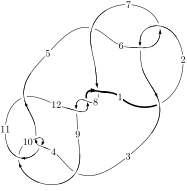
\includegraphics[width=112pt]{../../../GIT/diagram.site/Diagrams/png/1185_12a_0384.png}\\
\ \ \ A knot diagram\footnotemark}&
\allowdisplaybreaks
\textbf{Linearized knot diagam} \\
\cline{2-2}
 &
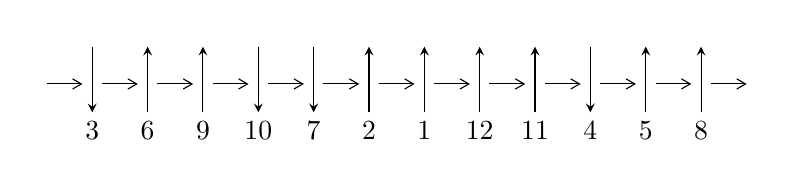
\begin{tikzpicture}[x=20pt, y=17pt]
	% nodes
	\node (C0) at (0, 0) {};
	\node (C1) at (1, 0) {};
	\node (C1U) at (1, +1) {};
	\node (C1D) at (1, -1) {3};

	\node (C2) at (2, 0) {};
	\node (C2U) at (2, +1) {};
	\node (C2D) at (2, -1) {6};

	\node (C3) at (3, 0) {};
	\node (C3U) at (3, +1) {};
	\node (C3D) at (3, -1) {9};

	\node (C4) at (4, 0) {};
	\node (C4U) at (4, +1) {};
	\node (C4D) at (4, -1) {10};

	\node (C5) at (5, 0) {};
	\node (C5U) at (5, +1) {};
	\node (C5D) at (5, -1) {7};

	\node (C6) at (6, 0) {};
	\node (C6U) at (6, +1) {};
	\node (C6D) at (6, -1) {2};

	\node (C7) at (7, 0) {};
	\node (C7U) at (7, +1) {};
	\node (C7D) at (7, -1) {1};

	\node (C8) at (8, 0) {};
	\node (C8U) at (8, +1) {};
	\node (C8D) at (8, -1) {12};

	\node (C9) at (9, 0) {};
	\node (C9U) at (9, +1) {};
	\node (C9D) at (9, -1) {11};

	\node (C10) at (10, 0) {};
	\node (C10U) at (10, +1) {};
	\node (C10D) at (10, -1) {4};

	\node (C11) at (11, 0) {};
	\node (C11U) at (11, +1) {};
	\node (C11D) at (11, -1) {5};

	\node (C12) at (12, 0) {};
	\node (C12U) at (12, +1) {};
	\node (C12D) at (12, -1) {8};
	\node (C13) at (13, 0) {};

	% arrows
	\draw[->,>={angle 60}]
	(C0) edge (C1) (C1) edge (C2) (C2) edge (C3) (C3) edge (C4) (C4) edge (C5) (C5) edge (C6) (C6) edge (C7) (C7) edge (C8) (C8) edge (C9) (C9) edge (C10) (C10) edge (C11) (C11) edge (C12) (C12) edge (C13) ;	\draw[->,>=stealth]
	(C1U) edge (C1D) (C2D) edge (C2U) (C3D) edge (C3U) (C4U) edge (C4D) (C5U) edge (C5D) (C6D) edge (C6U) (C7D) edge (C7U) (C8D) edge (C8U) (C9D) edge (C9U) (C10U) edge (C10D) (C11D) edge (C11U) (C12D) edge (C12U) ;
	\end{tikzpicture} \\
\hhline{~~} \\& 
\textbf{Solving Sequence} \\ \cline{2-2} 
 &
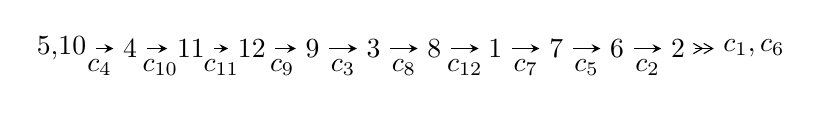
\begin{tikzpicture}[x=22pt, y=7pt]
	% node
	\node (A0) at (-1/8, 0) {5,10};
	\node (A1) at (1, 0) {4};
	\node (A2) at (2, 0) {11};
	\node (A3) at (3, 0) {12};
	\node (A4) at (4, 0) {9};
	\node (A5) at (5, 0) {3};
	\node (A6) at (6, 0) {8};
	\node (A7) at (7, 0) {1};
	\node (A8) at (8, 0) {7};
	\node (A9) at (9, 0) {6};
	\node (A10) at (10, 0) {2};
	\node (C1) at (1/2, -1) {$c_{4}$};
	\node (C2) at (3/2, -1) {$c_{10}$};
	\node (C3) at (5/2, -1) {$c_{11}$};
	\node (C4) at (7/2, -1) {$c_{9}$};
	\node (C5) at (9/2, -1) {$c_{3}$};
	\node (C6) at (11/2, -1) {$c_{8}$};
	\node (C7) at (13/2, -1) {$c_{12}$};
	\node (C8) at (15/2, -1) {$c_{7}$};
	\node (C9) at (17/2, -1) {$c_{5}$};
	\node (C10) at (19/2, -1) {$c_{2}$};
	\node (A11) at (45/4, 0) {$c_{1},c_{6}$};

	% edge
	\draw[->,>=stealth]	
	(A0) edge (A1) (A1) edge (A2) (A2) edge (A3) (A3) edge (A4) (A4) edge (A5) (A5) edge (A6) (A6) edge (A7) (A7) edge (A8) (A8) edge (A9) (A9) edge (A10) ;
	\draw[->>,>={angle 60}]	
	(A10) edge (A11);
\end{tikzpicture} \\ 

\end{tabular} \\

\footnotetext{
The image of knot diagram is generated by the software ``\textbf{Draw programme}" developed by Andrew Bartholomew(\url{http://www.layer8.co.uk/maths/draw/index.htm\#Running-draw}), where we modified some parts for our purpose(\url{https://github.com/CATsTAILs/LinksPainter}).
}\phantom \\ \newline 
\centering \textbf{Ideals for irreducible components\footnotemark of $X_{\text{par}}$} 
 
\begin{align*}
I^u_{1}&=\langle 
u^{75}- u^{74}+\cdots- u^2-1\rangle \\
\\
\end{align*}
\raggedright * 1 irreducible components of $\dim_{\mathbb{C}}=0$, with total 75 representations.\\
\footnotetext{All coefficients of polynomials are rational numbers. But the coefficients are sometimes approximated in decimal forms when there is not enough margin.}
\newpage
\renewcommand{\arraystretch}{1}
\centering \section*{I. $I^u_{1}= \langle u^{75}- u^{74}+\cdots- u^2-1 \rangle$}
\flushleft \textbf{(i) Arc colorings}\\
\begin{tabular}{m{7pt} m{180pt} m{7pt} m{180pt} }
\flushright $a_{5}=$&$\begin{pmatrix}1\\0\end{pmatrix}$ \\
\flushright $a_{10}=$&$\begin{pmatrix}0\\u\end{pmatrix}$ \\
\flushright $a_{4}=$&$\begin{pmatrix}1\\- u^2\end{pmatrix}$ \\
\flushright $a_{11}=$&$\begin{pmatrix}- u\\u^3+u\end{pmatrix}$ \\
\flushright $a_{12}=$&$\begin{pmatrix}u^3\\u^3+u\end{pmatrix}$ \\
\flushright $a_{9}=$&$\begin{pmatrix}- u^3\\u^5+u^3+u\end{pmatrix}$ \\
\flushright $a_{3}=$&$\begin{pmatrix}- u^6- u^4+1\\u^8+2 u^6+2 u^4\end{pmatrix}$ \\
\flushright $a_{8}=$&$\begin{pmatrix}- u^{11}-2 u^9-2 u^7- u^3\\- u^{11}-3 u^9-4 u^7- u^5+u^3+u\end{pmatrix}$ \\
\flushright $a_{1}=$&$\begin{pmatrix}u^{19}+4 u^{17}+8 u^{15}+8 u^{13}+5 u^{11}+2 u^9+2 u^7+u^3\\u^{19}+5 u^{17}+12 u^{15}+15 u^{13}+9 u^{11}- u^9-4 u^7-2 u^5+u^3+u\end{pmatrix}$ \\
\flushright $a_{7}=$&$\begin{pmatrix}- u^{27}-6 u^{25}+\cdots-4 u^7- u^3\\- u^{27}-7 u^{25}+\cdots+u^3+u\end{pmatrix}$ \\
\flushright $a_{6}=$&$\begin{pmatrix}u^{54}+13 u^{52}+\cdots- u^4+1\\u^{54}+14 u^{52}+\cdots+2 u^4+u^2\end{pmatrix}$ \\
\flushright $a_{2}=$&$\begin{pmatrix}- u^{33}-8 u^{31}+\cdots+4 u^5- u\\u^{35}+9 u^{33}+\cdots+u^3+u\end{pmatrix}$\\&\end{tabular}
\flushleft \textbf{(ii) Obstruction class $= -1$}\\~\\
\flushleft \textbf{(iii) Cusp Shapes $= -4 u^{73}+4 u^{72}+\cdots+8 u^2+6$}\\~\\
\newpage\renewcommand{\arraystretch}{1}
\flushleft \textbf{(iv) u-Polynomials at the component}\newline \\
\begin{tabular}{m{50pt}|m{274pt}}
Crossings & \hspace{64pt}u-Polynomials at each crossing \\
\hline $$\begin{aligned}c_{1},c_{5}\end{aligned}$$&$\begin{aligned}
&u^{75}+27 u^{74}+\cdots-2 u-1
\end{aligned}$\\
\hline $$\begin{aligned}c_{2},c_{6}\end{aligned}$$&$\begin{aligned}
&u^{75}- u^{74}+\cdots+2 u-1
\end{aligned}$\\
\hline $$\begin{aligned}c_{3},c_{11}\end{aligned}$$&$\begin{aligned}
&u^{75}+u^{74}+\cdots+224 u-37
\end{aligned}$\\
\hline $$\begin{aligned}c_{4},c_{10}\end{aligned}$$&$\begin{aligned}
&u^{75}- u^{74}+\cdots- u^2-1
\end{aligned}$\\
\hline $$\begin{aligned}c_{7},c_{8},c_{12}\end{aligned}$$&$\begin{aligned}
&u^{75}+5 u^{74}+\cdots-122 u-13
\end{aligned}$\\
\hline $$\begin{aligned}c_{9}\end{aligned}$$&$\begin{aligned}
&u^{75}-39 u^{74}+\cdots-2 u+1
\end{aligned}$\\
\hline
\end{tabular}\\~\\
\newpage\renewcommand{\arraystretch}{1}
\flushleft \textbf{(v) Riley Polynomials at the component}\newline \\
\begin{tabular}{m{50pt}|m{274pt}}
Crossings & \hspace{64pt}Riley Polynomials at each crossing \\
\hline $$\begin{aligned}c_{1},c_{5}\end{aligned}$$&$\begin{aligned}
&y^{75}+43 y^{74}+\cdots-42 y-1
\end{aligned}$\\
\hline $$\begin{aligned}c_{2},c_{6}\end{aligned}$$&$\begin{aligned}
&y^{75}+27 y^{74}+\cdots-2 y-1
\end{aligned}$\\
\hline $$\begin{aligned}c_{3},c_{11}\end{aligned}$$&$\begin{aligned}
&y^{75}-49 y^{74}+\cdots-139634 y-1369
\end{aligned}$\\
\hline $$\begin{aligned}c_{4},c_{10}\end{aligned}$$&$\begin{aligned}
&y^{75}+39 y^{74}+\cdots-2 y-1
\end{aligned}$\\
\hline $$\begin{aligned}c_{7},c_{8},c_{12}\end{aligned}$$&$\begin{aligned}
&y^{75}+71 y^{74}+\cdots+818 y-169
\end{aligned}$\\
\hline $$\begin{aligned}c_{9}\end{aligned}$$&$\begin{aligned}
&y^{75}-5 y^{74}+\cdots+6 y-1
\end{aligned}$\\
\hline
\end{tabular}\\~\\
\newpage\flushleft \textbf{(vi) Complex Volumes and Cusp Shapes}
$$\begin{array}{c|c|c}  
\text{Solutions to }I^u_{1}& \I (\text{vol} + \sqrt{-1}CS) & \text{Cusp shape}\\
 \hline 
\begin{aligned}
u &= -0.605676 + 0.796769 I\end{aligned}
 & -6.04317 + 9.23163 I & \phantom{-0.000000 } 0. - 8.30449 I \\ \hline\begin{aligned}
u &= -0.605676 - 0.796769 I\end{aligned}
 & -6.04317 - 9.23163 I & \phantom{-0.000000 -}0. + 8.30449 I \\ \hline\begin{aligned}
u &= \phantom{-}0.434200 + 0.904835 I\end{aligned}
 & \phantom{-}1.00534 - 6.47824 I & \phantom{-}4.00000 + 9.67055 I \\ \hline\begin{aligned}
u &= \phantom{-}0.434200 - 0.904835 I\end{aligned}
 & \phantom{-}1.00534 + 6.47824 I & \phantom{-}4.00000 - 9.67055 I \\ \hline\begin{aligned}
u &= -0.357332 + 0.925036 I\end{aligned}
 & \phantom{-}1.74821 + 1.50345 I & \phantom{-}6.59382 - 3.63022 I \\ \hline\begin{aligned}
u &= -0.357332 - 0.925036 I\end{aligned}
 & \phantom{-}1.74821 - 1.50345 I & \phantom{-}6.59382 + 3.63022 I \\ \hline\begin{aligned}
u &= \phantom{-}0.596114 + 0.790314 I\end{aligned}
 & -4.52032 - 3.81412 I & \phantom{-}1.55948 + 3.68783 I \\ \hline\begin{aligned}
u &= \phantom{-}0.596114 - 0.790314 I\end{aligned}
 & -4.52032 + 3.81412 I & \phantom{-}1.55948 - 3.68783 I \\ \hline\begin{aligned}
u &= -0.611709 + 0.774118 I\end{aligned}
 & -10.27490 + 2.38694 I & -4.63689 - 3.32182 I \\ \hline\begin{aligned}
u &= -0.611709 - 0.774118 I\end{aligned}
 & -10.27490 - 2.38694 I & -4.63689 + 3.32182 I \\ \hline\begin{aligned}
u &= -0.611730 + 0.749244 I\end{aligned}
 & -6.17981 - 4.47538 I & -0.99002 + 1.78684 I \\ \hline\begin{aligned}
u &= -0.611730 - 0.749244 I\end{aligned}
 & -6.17981 + 4.47538 I & -0.99002 - 1.78684 I \\ \hline\begin{aligned}
u &= \phantom{-}0.599256 + 0.754022 I\end{aligned}
 & -4.62446 - 0.87914 I & \phantom{-}1.19980 + 3.06129 I \\ \hline\begin{aligned}
u &= \phantom{-}0.599256 - 0.754022 I\end{aligned}
 & -4.62446 + 0.87914 I & \phantom{-}1.19980 - 3.06129 I \\ \hline\begin{aligned}
u &= -0.026354 + 0.944514 I\end{aligned}
 & \phantom{-}3.78137 + 2.60614 I & \phantom{-}11.97414 - 3.59156 I \\ \hline\begin{aligned}
u &= -0.026354 - 0.944514 I\end{aligned}
 & \phantom{-}3.78137 - 2.60614 I & \phantom{-}11.97414 + 3.59156 I \\ \hline\begin{aligned}
u &= \phantom{-}0.445777 + 0.744877 I\end{aligned}
 & -2.71406 - 1.90275 I & -3.96566 + 4.94031 I \\ \hline\begin{aligned}
u &= \phantom{-}0.445777 - 0.744877 I\end{aligned}
 & -2.71406 + 1.90275 I & -3.96566 - 4.94031 I \\ \hline\begin{aligned}
u &= \phantom{-}0.297220 + 1.135960 I\end{aligned}
 & \phantom{-}0.31557 - 6.14170 I & \phantom{-0.000000 } 0 \\ \hline\begin{aligned}
u &= \phantom{-}0.297220 - 1.135960 I\end{aligned}
 & \phantom{-}0.31557 + 6.14170 I & \phantom{-0.000000 } 0 \\ \hline\begin{aligned}
u &= \phantom{-}0.792174 + 0.211922 I\end{aligned}
 & -3.19444 + 10.59060 I & \phantom{-}1.16244 - 7.05944 I \\ \hline\begin{aligned}
u &= \phantom{-}0.792174 - 0.211922 I\end{aligned}
 & -3.19444 - 10.59060 I & \phantom{-}1.16244 + 7.05944 I \\ \hline\begin{aligned}
u &= -0.326975 + 1.136760 I\end{aligned}
 & \phantom{-}1.78383 + 1.05705 I & \phantom{-0.000000 } 0 \\ \hline\begin{aligned}
u &= -0.326975 - 1.136760 I\end{aligned}
 & \phantom{-}1.78383 - 1.05705 I & \phantom{-0.000000 } 0 \\ \hline\begin{aligned}
u &= \phantom{-}0.778680 + 0.229580 I\end{aligned}
 & -7.67564 + 3.86014 I & -3.36188 - 2.54547 I \\ \hline\begin{aligned}
u &= \phantom{-}0.778680 - 0.229580 I\end{aligned}
 & -7.67564 - 3.86014 I & -3.36188 + 2.54547 I \\ \hline\begin{aligned}
u &= -0.783246 + 0.208394 I\end{aligned}
 & -1.76009 - 5.07972 I & \phantom{-}3.22251 + 2.55358 I \\ \hline\begin{aligned}
u &= -0.783246 - 0.208394 I\end{aligned}
 & -1.76009 + 5.07972 I & \phantom{-}3.22251 - 2.55358 I \\ \hline\begin{aligned}
u &= -0.416318 + 1.118240 I\end{aligned}
 & \phantom{-}2.27451 + 1.40801 I & \phantom{-0.000000 } 0 \\ \hline\begin{aligned}
u &= -0.416318 - 1.118240 I\end{aligned}
 & \phantom{-}2.27451 - 1.40801 I & \phantom{-0.000000 } 0\\
 \hline 
 \end{array}$$\newpage$$\begin{array}{c|c|c}  
\text{Solutions to }I^u_{1}& \I (\text{vol} + \sqrt{-1}CS) & \text{Cusp shape}\\
 \hline 
\begin{aligned}
u &= \phantom{-}0.756757 + 0.247164 I\end{aligned}
 & -3.87573 - 2.95735 I & -0.06195 + 2.67044 I \\ \hline\begin{aligned}
u &= \phantom{-}0.756757 - 0.247164 I\end{aligned}
 & -3.87573 + 2.95735 I & -0.06195 - 2.67044 I \\ \hline\begin{aligned}
u &= \phantom{-}0.312742 + 1.169010 I\end{aligned}
 & -3.42309 + 0.45321 I & \phantom{-0.000000 } 0 \\ \hline\begin{aligned}
u &= \phantom{-}0.312742 - 1.169010 I\end{aligned}
 & -3.42309 - 0.45321 I & \phantom{-0.000000 } 0 \\ \hline\begin{aligned}
u &= -0.752182 + 0.229843 I\end{aligned}
 & -2.28210 - 2.23283 I & \phantom{-}2.43604 + 2.41048 I \\ \hline\begin{aligned}
u &= -0.752182 - 0.229843 I\end{aligned}
 & -2.28210 + 2.23283 I & \phantom{-}2.43604 - 2.41048 I \\ \hline\begin{aligned}
u &= -0.331893 + 1.180670 I\end{aligned}
 & \phantom{-}2.43376 - 1.52363 I & \phantom{-0.000000 } 0 \\ \hline\begin{aligned}
u &= -0.331893 - 1.180670 I\end{aligned}
 & \phantom{-}2.43376 + 1.52363 I & \phantom{-0.000000 } 0 \\ \hline\begin{aligned}
u &= \phantom{-}0.325952 + 1.187250 I\end{aligned}
 & \phantom{-}1.06510 + 7.02113 I & \phantom{-0.000000 } 0 \\ \hline\begin{aligned}
u &= \phantom{-}0.325952 - 1.187250 I\end{aligned}
 & \phantom{-}1.06510 - 7.02113 I & \phantom{-0.000000 } 0 \\ \hline\begin{aligned}
u &= -0.214391 + 0.731240 I\end{aligned}
 & \phantom{-}0.447274 + 1.029570 I & \phantom{-}6.61766 - 6.37411 I \\ \hline\begin{aligned}
u &= -0.214391 - 0.731240 I\end{aligned}
 & \phantom{-}0.447274 - 1.029570 I & \phantom{-}6.61766 + 6.37411 I \\ \hline\begin{aligned}
u &= \phantom{-}0.449541 + 1.154810 I\end{aligned}
 & \phantom{-}4.51193 - 4.07458 I & \phantom{-0.000000 } 0 \\ \hline\begin{aligned}
u &= \phantom{-}0.449541 - 1.154810 I\end{aligned}
 & \phantom{-}4.51193 + 4.07458 I & \phantom{-0.000000 } 0 \\ \hline\begin{aligned}
u &= -0.482271 + 1.142580 I\end{aligned}
 & \phantom{-}1.76946 + 6.42913 I & \phantom{-0.000000 } 0 \\ \hline\begin{aligned}
u &= -0.482271 - 1.142580 I\end{aligned}
 & \phantom{-}1.76946 - 6.42913 I & \phantom{-0.000000 } 0 \\ \hline\begin{aligned}
u &= -0.751767 + 0.088561 I\end{aligned}
 & \phantom{-}3.83758 - 5.79700 I & \phantom{-}6.35953 + 6.44372 I \\ \hline\begin{aligned}
u &= -0.751767 - 0.088561 I\end{aligned}
 & \phantom{-}3.83758 + 5.79700 I & \phantom{-}6.35953 - 6.44372 I \\ \hline\begin{aligned}
u &= \phantom{-}0.744452 + 0.066574 I\end{aligned}
 & \phantom{-}4.31968 + 0.36674 I & \phantom{-}7.87220 - 0.50275 I \\ \hline\begin{aligned}
u &= \phantom{-}0.744452 - 0.066574 I\end{aligned}
 & \phantom{-}4.31968 - 0.36674 I & \phantom{-}7.87220 + 0.50275 I \\ \hline\begin{aligned}
u &= -0.409035 + 1.184990 I\end{aligned}
 & \phantom{-}7.51694 - 1.78430 I & \phantom{-0.000000 } 0 \\ \hline\begin{aligned}
u &= -0.409035 - 1.184990 I\end{aligned}
 & \phantom{-}7.51694 + 1.78430 I & \phantom{-0.000000 } 0 \\ \hline\begin{aligned}
u &= \phantom{-}0.419688 + 1.183890 I\end{aligned}
 & \phantom{-}7.91319 - 3.70818 I & \phantom{-0.000000 } 0 \\ \hline\begin{aligned}
u &= \phantom{-}0.419688 - 1.183890 I\end{aligned}
 & \phantom{-}7.91319 + 3.70818 I & \phantom{-0.000000 } 0 \\ \hline\begin{aligned}
u &= \phantom{-}0.533487 + 1.149800 I\end{aligned}
 & -1.23150 - 1.88454 I & \phantom{-0.000000 } 0 \\ \hline\begin{aligned}
u &= \phantom{-}0.533487 - 1.149800 I\end{aligned}
 & -1.23150 + 1.88454 I & \phantom{-0.000000 } 0 \\ \hline\begin{aligned}
u &= -0.527390 + 1.154690 I\end{aligned}
 & \phantom{-}0.42284 + 7.03628 I & \phantom{-0.000000 } 0 \\ \hline\begin{aligned}
u &= -0.527390 - 1.154690 I\end{aligned}
 & \phantom{-}0.42284 - 7.03628 I & \phantom{-0.000000 } 0 \\ \hline\begin{aligned}
u &= \phantom{-}0.474033 + 1.180990 I\end{aligned}
 & \phantom{-}7.52996 - 4.83567 I & \phantom{-0.000000 } 0 \\ \hline\begin{aligned}
u &= \phantom{-}0.474033 - 1.180990 I\end{aligned}
 & \phantom{-}7.52996 + 4.83567 I & \phantom{-0.000000 } 0\\
 \hline 
 \end{array}$$\newpage$$\begin{array}{c|c|c}  
\text{Solutions to }I^u_{1}& \I (\text{vol} + \sqrt{-1}CS) & \text{Cusp shape}\\
 \hline 
\begin{aligned}
u &= -0.482557 + 1.181340 I\end{aligned}
 & \phantom{-}6.99960 + 10.33920 I & \phantom{-0.000000 } 0 \\ \hline\begin{aligned}
u &= -0.482557 - 1.181340 I\end{aligned}
 & \phantom{-}6.99960 - 10.33920 I & \phantom{-0.000000 } 0 \\ \hline\begin{aligned}
u &= \phantom{-}0.535680 + 1.162020 I\end{aligned}
 & -4.93464 - 8.76118 I & \phantom{-0.000000 } 0 \\ \hline\begin{aligned}
u &= \phantom{-}0.535680 - 1.162020 I\end{aligned}
 & -4.93464 + 8.76118 I & \phantom{-0.000000 } 0 \\ \hline\begin{aligned}
u &= -0.530550 + 1.169690 I\end{aligned}
 & \phantom{-}1.06556 + 9.96571 I & \phantom{-0.000000 } 0 \\ \hline\begin{aligned}
u &= -0.530550 - 1.169690 I\end{aligned}
 & \phantom{-}1.06556 - 9.96571 I & \phantom{-0.000000 } 0 \\ \hline\begin{aligned}
u &= \phantom{-}0.534111 + 1.171560 I\end{aligned}
 & -0.3673 - 15.5144 I & \phantom{-0.000000 } 0 \\ \hline\begin{aligned}
u &= \phantom{-}0.534111 - 1.171560 I\end{aligned}
 & -0.3673 + 15.5144 I & \phantom{-0.000000 } 0 \\ \hline\begin{aligned}
u &= \phantom{-}0.458828 + 0.536244 I\end{aligned}
 & -0.03059 + 2.65332 I & -0.13467 - 2.90348 I \\ \hline\begin{aligned}
u &= \phantom{-}0.458828 - 0.536244 I\end{aligned}
 & -0.03059 - 2.65332 I & -0.13467 + 2.90348 I \\ \hline\begin{aligned}
u &= -0.646867 + 0.153322 I\end{aligned}
 & -1.02159 - 2.08911 I & -1.37094 + 4.75504 I \\ \hline\begin{aligned}
u &= -0.646867 - 0.153322 I\end{aligned}
 & -1.02159 + 2.08911 I & -1.37094 - 4.75504 I \\ \hline\begin{aligned}
u &= \phantom{-}0.651127\phantom{ +0.000000I}\end{aligned}
 & \phantom{-}1.36435\phantom{ +0.000000I} & \phantom{-}8.10100\phantom{ +0.000000I} \\ \hline\begin{aligned}
u &= -0.446014 + 0.404386 I\end{aligned}
 & \phantom{-}0.26212 + 1.94827 I & \phantom{-}0.25758 - 3.35365 I \\ \hline\begin{aligned}
u &= -0.446014 - 0.404386 I\end{aligned}
 & \phantom{-}0.26212 - 1.94827 I & \phantom{-}0.25758 + 3.35365 I\\
 \hline 
 \end{array}$$\newpage
\newpage\renewcommand{\arraystretch}{1}
\centering \section*{ II. u-Polynomials}
\begin{tabular}{m{50pt}|m{274pt}}
Crossings & \hspace{64pt}u-Polynomials at each crossing \\
\hline $$\begin{aligned}c_{1},c_{5}\end{aligned}$$&$\begin{aligned}
&u^{75}+27 u^{74}+\cdots-2 u-1
\end{aligned}$\\
\hline $$\begin{aligned}c_{2},c_{6}\end{aligned}$$&$\begin{aligned}
&u^{75}- u^{74}+\cdots+2 u-1
\end{aligned}$\\
\hline $$\begin{aligned}c_{3},c_{11}\end{aligned}$$&$\begin{aligned}
&u^{75}+u^{74}+\cdots+224 u-37
\end{aligned}$\\
\hline $$\begin{aligned}c_{4},c_{10}\end{aligned}$$&$\begin{aligned}
&u^{75}- u^{74}+\cdots- u^2-1
\end{aligned}$\\
\hline $$\begin{aligned}c_{7},c_{8},c_{12}\end{aligned}$$&$\begin{aligned}
&u^{75}+5 u^{74}+\cdots-122 u-13
\end{aligned}$\\
\hline $$\begin{aligned}c_{9}\end{aligned}$$&$\begin{aligned}
&u^{75}-39 u^{74}+\cdots-2 u+1
\end{aligned}$\\
\hline
\end{tabular}\newpage\renewcommand{\arraystretch}{1}
\centering \section*{ III. Riley Polynomials}
\begin{tabular}{m{50pt}|m{274pt}}
Crossings & \hspace{64pt}Riley Polynomials at each crossing \\
\hline $$\begin{aligned}c_{1},c_{5}\end{aligned}$$&$\begin{aligned}
&y^{75}+43 y^{74}+\cdots-42 y-1
\end{aligned}$\\
\hline $$\begin{aligned}c_{2},c_{6}\end{aligned}$$&$\begin{aligned}
&y^{75}+27 y^{74}+\cdots-2 y-1
\end{aligned}$\\
\hline $$\begin{aligned}c_{3},c_{11}\end{aligned}$$&$\begin{aligned}
&y^{75}-49 y^{74}+\cdots-139634 y-1369
\end{aligned}$\\
\hline $$\begin{aligned}c_{4},c_{10}\end{aligned}$$&$\begin{aligned}
&y^{75}+39 y^{74}+\cdots-2 y-1
\end{aligned}$\\
\hline $$\begin{aligned}c_{7},c_{8},c_{12}\end{aligned}$$&$\begin{aligned}
&y^{75}+71 y^{74}+\cdots+818 y-169
\end{aligned}$\\
\hline $$\begin{aligned}c_{9}\end{aligned}$$&$\begin{aligned}
&y^{75}-5 y^{74}+\cdots+6 y-1
\end{aligned}$\\
\hline
\end{tabular}
\vskip 2pc
\end{document}